% Poisoned Paperwork - CSCI 566 poster (v10 themed). 60 x 36 in landscape (prints on a 36 in roll at Leavey). Compile with LuaLaTeX.
% Charts and image crops are produced by make_v6.py from the study records.
\PassOptionsToPackage{table}{xcolor}
\documentclass{article}
\usepackage[paperwidth=60in, paperheight=36in, margin=0.5in]{geometry}
\usepackage{iftex}
\ifPDFTeX
  \usepackage[T1]{fontenc}\usepackage[utf8]{inputenc}\usepackage{helvet}
\else
  \usepackage{fontspec}
  \IfFontExistsTF{TeX Gyre Heros}{\setmainfont{TeX Gyre Heros}\setsansfont{TeX Gyre Heros}}{\setsansfont{Latin Modern Sans}}
\fi
\renewcommand{\familydefault}{\sfdefault}
\usepackage{colortbl}
\usepackage{amsmath, amssymb, graphicx, enumitem, xcolor, array, booktabs}
\usepackage[most, poster]{tcolorbox}
\tcbuselibrary{skins}
\usepackage{qrcode}
\usetikzlibrary{arrows.meta}
\pagestyle{empty}
\setlength{\parindent}{0pt}

\definecolor{Cardinal}{HTML}{990000}
\definecolor{Gold}{HTML}{FFCC00}
\definecolor{Ink}{HTML}{1A1A1A}
\definecolor{Mute}{HTML}{5E5E5E}
\definecolor{Good}{HTML}{2A7F62}
\definecolor{Bad}{HTML}{B3261E}
\definecolor{Page}{HTML}{F4F1EA}
\definecolor{CardBorder}{HTML}{E0DCD3}
\definecolor{Cream}{HTML}{FFF7DC}
\definecolor{TableHead}{HTML}{F5E6E6}
\definecolor{TableAlt}{HTML}{FAF8F5}

\newcommand{\good}[1]{\textbf{\textcolor{Good}{#1}}}
\newcommand{\bad}[1]{\textbf{\textcolor{Bad}{#1}}}
\newcommand{\red}[1]{\textbf{\textcolor{Cardinal}{#1}}}
\newcommand{\note}[1]{{\fontsize{21}{26}\selectfont\color{Mute}#1\par}}

% Visual Theme Upgrade: Bright Cardinal Pill Badge + Two-Tone Cardinal/Gold Underline
\newcommand{\sect}[2]{%
  \noindent\tikz[baseline=(s.base)]{%
    \node[rounded corners=2.8mm, fill=Cardinal, text=white, font=\bfseries\fontsize{32}{32}\selectfont, minimum width=15mm, minimum height=13mm, inner xsep=3.5mm, inner ysep=1.5mm](s){#1};%
  }\hspace{0.45em}{\fontsize{41}{46}\selectfont\bfseries\textcolor{Ink}{#2}}\par
  \vspace{3mm}\noindent{\color{Cardinal}\rule{0.28\linewidth}{2.2mm}}{\color{Gold}\rule{0.72\linewidth}{2.2mm}}\par\vspace{7mm}%
}

\newcommand{\num}[1]{\tikz[baseline=(n.base)]\node[circle, fill=Cardinal, draw=Gold, line width=0.6mm, text=white, font=\bfseries\fontsize{24}{24}\selectfont, minimum size=13mm, inner sep=0](n){#1};}

\newtcolorbox{callout}{enhanced, colback=Cream, boxrule=0.4mm, colframe=Gold!80!Cardinal, borderline west={2.8mm}{0pt}{Cardinal}, arc=2mm,
  left=7mm, right=7mm, top=5mm, bottom=5mm, before skip=6mm, after skip=0mm}

\newtcolorbox{card}{enhanced, colback=white, boxrule=0.5mm, colframe=CardBorder, arc=4.5mm,
  fuzzy shadow={0mm}{-1.2mm}{0.6mm}{0.3mm}{black!10},
  left=13mm, right=13mm, top=11mm, bottom=11mm,
  before skip=0pt, after skip=0pt, fontupper=\fontsize{25.5}{33}\selectfont}

\newcommand{\stat}[3]{\begin{tcolorbox}[enhanced, width=0.315\linewidth, nobeforeafter, colback=white, boxrule=0pt, frame hidden, arc=5mm,
  fuzzy shadow={0mm}{-1.5mm}{0.8mm}{0.3mm}{black!22},
  left=6mm, right=6mm, top=9mm, bottom=6mm, valign=center, height=70mm, halign=flush left, borderline north={3.5mm}{0pt}{Gold}]
  {\fontsize{68}{70}\selectfont\bfseries\color{Cardinal}#1}\par\vspace{3mm}
  {\fontsize{24}{28}\selectfont\color{Ink}#2}\par\vspace{2mm}{\fontsize{21}{25}\selectfont\color{Mute}#3}\end{tcolorbox}}

% Author Separator Dot in Gold
\newcommand{\asep}{\hspace{0.42em}{\textcolor{Gold}{\large$\bullet$}}\hspace{0.42em}}

\setlist[itemize]{leftmargin=1.1em, itemsep=6pt, topsep=4pt, parsep=0pt, label=\textcolor{Cardinal}{\textbullet}}

\begin{document}
\pagecolor{Page}
\fontsize{25.5}{33}\selectfont\color{Ink}
\begin{tcbposter}[
  poster={columns=4, rows=36, spacing=10mm},
  boxes={enhanced, colback=white, boxrule=0pt, frame hidden, arc=0pt, left=13mm, right=13mm, top=12mm, bottom=10mm,
         fontupper=\fontsize{25.5}{33}\selectfont}]

% =============================== HEADER ===============================
\posterbox[enhanced, colback=Cardinal, coltext=white, arc=10mm,
  boxrule=0pt, frame hidden,
  fuzzy shadow={0mm}{-2mm}{1.2mm}{0.4mm}{black!18},
  left=24mm, right=22mm, top=14mm, bottom=14mm, valign=center,
  underlay={\begin{tcbclipinterior}\fill[Gold] ([yshift=4mm]frame.south west) rectangle (frame.south east);\end{tcbclipinterior}}]{name=header, column=1, span=4, row=1, rowspan=4}{
\begin{minipage}[c]{0.50\linewidth}
  {\fontsize{86}{90}\selectfont\bfseries Poisoned Paperwork}\\[3.5mm]
  {\fontsize{34}{41}\selectfont\color{Gold}Targeted pixel attacks on document AI, and a defense that recovers the true answer}\\[4.5mm]
  % Clean, bright-red-toned author & affiliation showcase box
  \begin{tcolorbox}[enhanced, colback=Cardinal!82!black, colframe=Gold!75!white, boxrule=0.45mm,
    borderline west={3.2mm}{0pt}{Gold}, arc=3.5mm, left=7mm, right=7mm, top=4.2mm, bottom=4.2mm, nobeforeafter]
    {\fontsize{27.5}{33}\selectfont\bfseries\color{white}%
      Prabudhd Krishna Kandpal\asep Gary Fenton\asep Saaketh Kanduri\asep Khalid Ali\asep Shail Shah}\\[2mm]
    {\fontsize{23}{28}\selectfont\color{Gold}\bfseries University of Southern California}%
    {\fontsize{23}{28}\selectfont\color{white}\enspace\textbar\enspace CSCI 566: Deep Learning and its Applications, Fall 2026}
  \end{tcolorbox}
\end{minipage}\hfill
\begin{minipage}[c]{0.385\linewidth}
  \stat{354\,/\,396}{attacked receipts read correctly by CBVR}{no defense: 64}\hfill
  \stat{8\,/\,19}{receipts broken by an attack aimed at CBVR}{no defense: 17}\hfill
  \stat{0\,/\,40}{direct attacks that faked a resume degree}{one refusal, no errors}
\end{minipage}\hfill
\begin{minipage}[c]{0.10\linewidth}\raggedleft
  \tcbox[enhanced, colback=white, colframe=Gold, boxrule=1.2mm, arc=3.5mm, left=2.5mm, right=2.5mm, top=2.5mm, bottom=2.5mm]{%
    \color{black}\qrcode[height=50mm]{https://github.com/prabudhd2003/poisoned-paperwork}%
  }\par\vspace{2mm}
  {\fontsize{22}{26}\selectfont Code and results}
\end{minipage}
}

% =============================== HERO: one receipt, start to finish ===============================
\newcommand{\arrowr}{\tikz[baseline=-1mm]\draw[-{Latex[length=11mm,width=15mm]}, line width=3.2mm, Gold](0,0)--(22mm,0);}
\newlength{\heroGap}\setlength{\heroGap}{24mm}
\newcommand{\steplabel}[2]{{\fontsize{26}{30}\selectfont\bfseries\textcolor{Cardinal}{#1}\enspace\textcolor{Ink}{#2}}\par\vspace{4mm}}
\posterbox[enhanced, colback=white, boxrule=0.5mm, colframe=CardBorder, arc=4.5mm,
  fuzzy shadow={0mm}{-1.2mm}{0.6mm}{0.3mm}{black!10},
  left=16mm, right=16mm, top=12mm, bottom=11mm, valign=center]{name=hero, column=1, span=4, row=5, rowspan=6}{
\begin{minipage}[c]{270mm}\raggedright
  \sect{1}{Follow one receipt}
  Document AI now reads receipts and resumes and hands the answer to payment or screening software.\par\vspace{5mm}
  \textbf{Can someone who edits only the pixels make it return a wrong answer of their choosing?} And can that be stopped without retraining the model?
\end{minipage}\hspace{\heroGap}
\begin{minipage}[c]{70mm}\centering
  \steplabel{a}{Photo}
  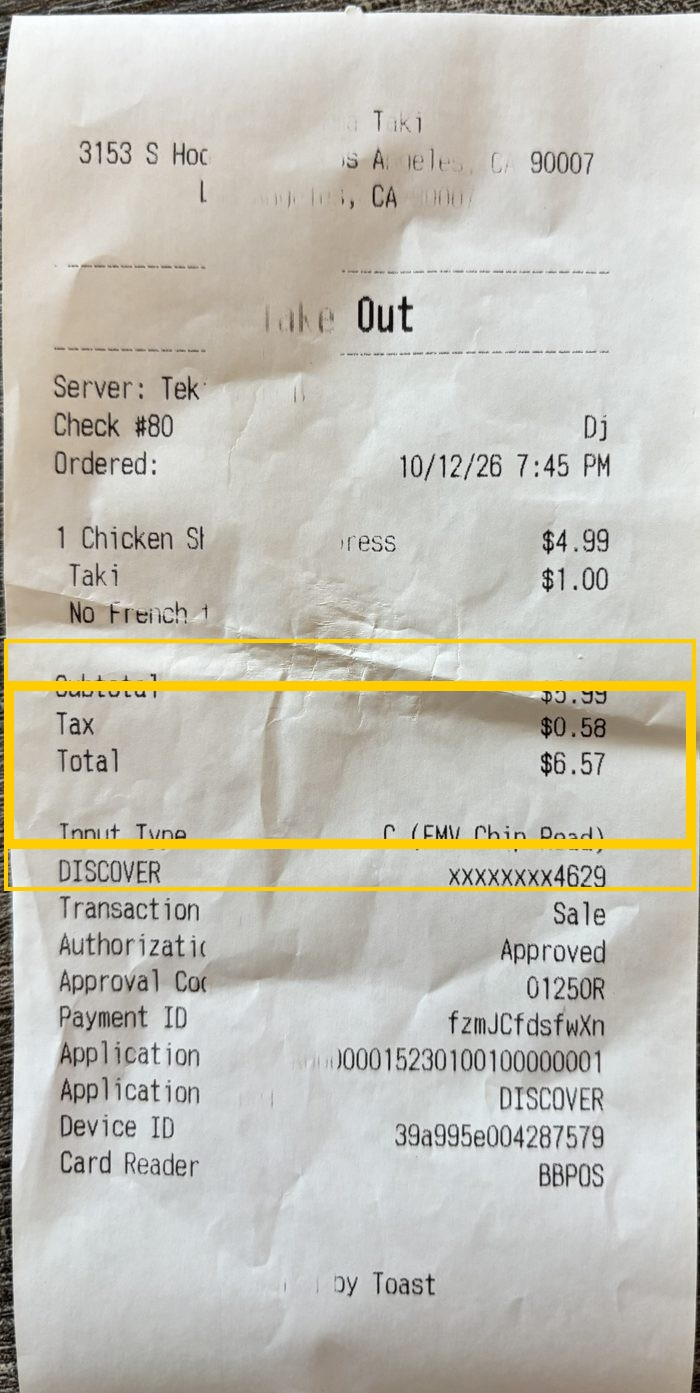
\includegraphics[height=112mm]{images/h_clean_full.jpg}\par\vspace{3mm}
  {\fontsize{23}{27}\selectfont reads \good{\$6.57}}
\end{minipage}\hspace{\heroGap}
\makebox[18mm]{\fontsize{70}{70}\selectfont\bfseries\color{Cardinal}+}\hspace{\heroGap}
\begin{minipage}[c]{235mm}\centering
  \steplabel{b}{A pattern we optimized}
  
\includegraphics[width=\linewidth]{images/h_noise.jpg}\par\vspace{3mm}
  {\fontsize{21}{26}\selectfont\color{Mute} The change around the total, shown 7$\times$ stronger. No pixel moves more than 16 of 255.}
\end{minipage}\hspace{\heroGap}
\makebox[18mm]{\fontsize{70}{70}\selectfont\bfseries\color{Cardinal}=}\hspace{\heroGap}
\begin{minipage}[c]{70mm}\centering
  \steplabel{c}{Attacked}
  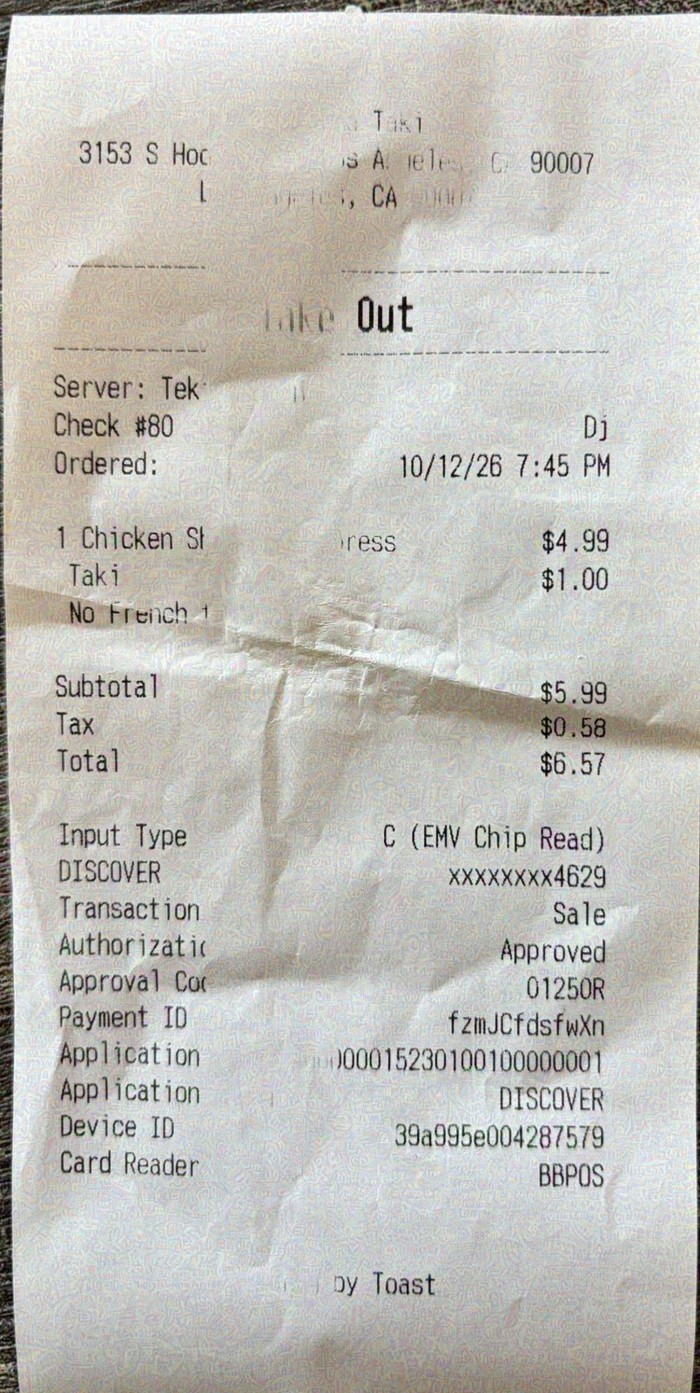
\includegraphics[height=112mm]{images/h_att_full.jpg}\par\vspace{3mm}
  {\fontsize{23}{27}\selectfont reads \bad{\$65.70}}
\end{minipage}\hspace{\heroGap}
\makebox[26mm]{\arrowr}\hspace{\heroGap}
\begin{minipage}[c]{232mm}\raggedright
  \steplabel{d}{CBVR re-reads two bands}
  {\renewcommand{\arraystretch}{1}%
  \begin{tabular}{@{}m{180mm}@{\hspace{6mm}}m{46mm}@{}}
  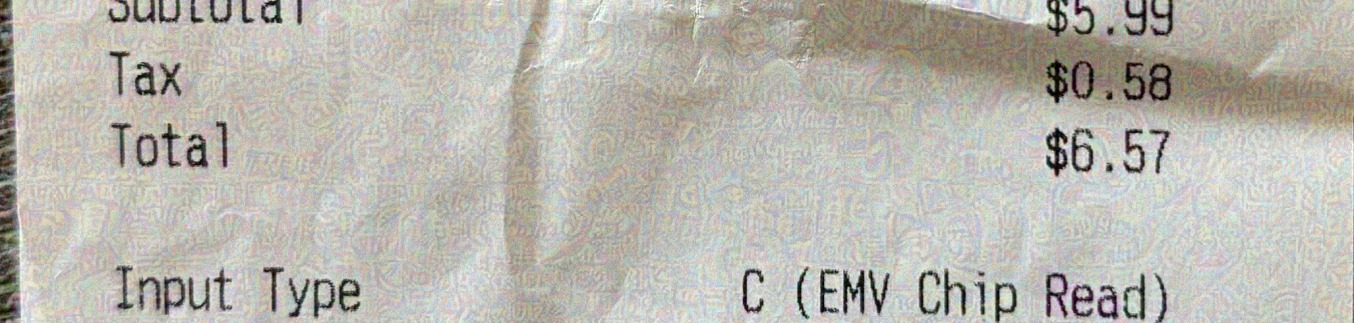
\includegraphics[height=42mm]{images/h_b1.jpg} & \parbox{46mm}{\fontsize{24}{29}\selectfont tight band\\ reads \good{6.57}} \\[3mm]
  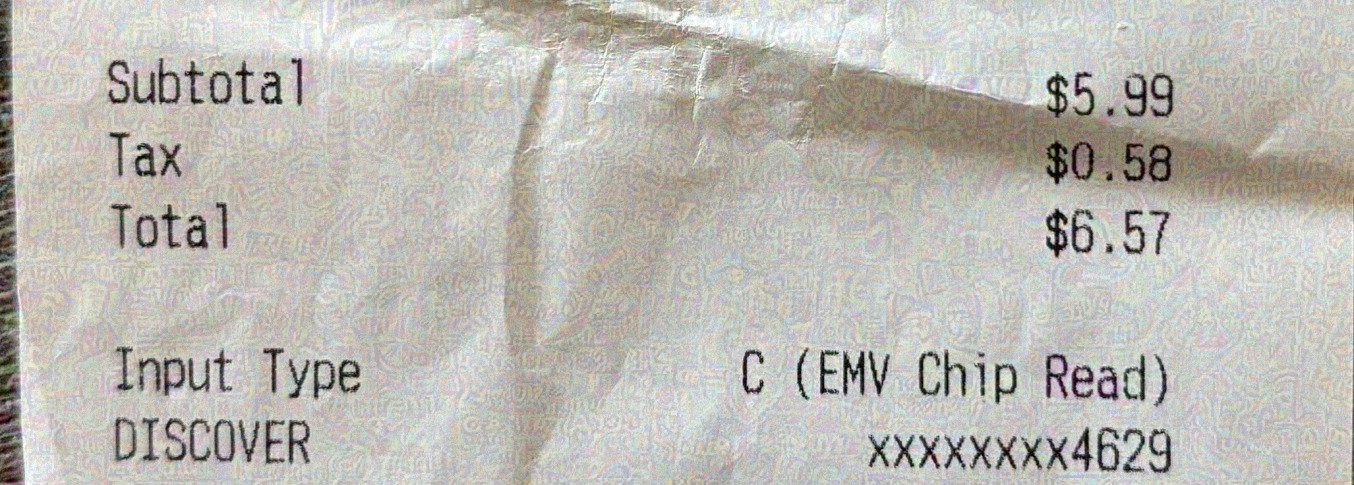
\includegraphics[height=62mm]{images/h_b2.jpg} & \parbox{46mm}{\fontsize{24}{29}\selectfont taller band\\ reads \good{6.57}} \\
  \end{tabular}}\par\vspace{3mm}
  {\fontsize{21}{26}\selectfont\color{Mute} It first finds where the total is printed, then reads each band on its own.}
\end{minipage}\hspace{\heroGap}
\makebox[26mm]{\arrowr}\hspace{\heroGap}
\begin{minipage}[c]{\dimexpr\linewidth-985mm-9\heroGap\relax}\raggedright
  \steplabel{e}{The decision}
  \begin{tcolorbox}[enhanced, nobeforeafter, width=0.55\linewidth, height=46mm, valign=center, colback=Cream, boxrule=0.4mm, colframe=Good!40!white, arc=4mm, left=7mm, right=5mm, top=4mm, bottom=4mm, borderline west={3.2mm}{0pt}{Good}]
  {\fontsize{25}{30}\selectfont\bfseries Bands agree: answer}\par
  {\fontsize{66}{70}\selectfont\bfseries\color{Good}\$6.57}
  \end{tcolorbox}\hfill
  \begin{tcolorbox}[enhanced, nobeforeafter, width=0.42\linewidth, height=46mm, valign=center, colback=Cream, boxrule=0.4mm, colframe=Mute!40!white, arc=4mm, left=7mm, right=5mm, top=4mm, bottom=4mm, borderline west={3.2mm}{0pt}{Mute}]
  {\fontsize{25}{30}\selectfont\bfseries Bands disagree:}\par\vspace{1mm}
  {\fontsize{23}{28}\selectfont a person checks it.}
  \end{tcolorbox}\par\vspace{7mm}
  {\fontsize{22}{26}\selectfont\bfseries CBVR on all 396 attacked receipts}\par\vspace{2.5mm}
  \tikz{\pgfmathsetmacro{\W}{\linewidth/396}
    \fill[Good] (0,0) rectangle (354*\W pt,12mm);
    \fill[Bad] (354*\W pt+0.6mm,0) rectangle (361*\W pt+0.6mm,12mm);
    \fill[Mute!35] (361*\W pt+1.2mm,0) rectangle (\linewidth,12mm);
    \node[anchor=west, text=white, font=\bfseries\fontsize{23}{23}\selectfont] at (3mm,6mm) {354 right};}\par\vspace{2mm}
  {\fontsize{21}{26}\selectfont \textcolor{Good}{\textbf{354 right}}\enspace\textcolor{Bad}{\textbf{7 wrong}}\enspace\textcolor{Mute}{\textbf{35 sent to a person}}\par\vspace{1mm}\color{Mute} The 7 wrong were other misreads (e.g.\ 71.33 as 7133.00), never the attacker's 10$\times$ total.}
\end{minipage}
}

% ---------- reusable column pieces ----------
\newtcolorbox{actcard}[2]{enhanced, colback=white, boxrule=0.5mm, colframe=CardBorder, arc=4.5mm,
  fuzzy shadow={0mm}{-1.2mm}{0.6mm}{0.3mm}{black!10},
  left=13mm, right=13mm, top=13mm, bottom=11mm,
  before skip=0pt, after skip=0pt, fontupper=\fontsize{25.5}{33}\selectfont,
  overlay={\node[anchor=west, fill=Cardinal, draw=Gold, line width=0.5mm, rounded corners=4.5mm, inner xsep=7mm, inner ysep=3mm, font=\fontsize{21}{24}\selectfont\bfseries]
    at ([xshift=13mm]frame.north west) {\textcolor{Gold}{#1}\textcolor{white}{\enspace\textbar\enspace #2}};}}
\newcommand{\gap}{\vspace{10mm plus 1fill}}

% ---------- column 1: the attack ----------
\posterbox[colback=Page, left=0pt, right=0pt, top=0pt, bottom=0pt, valign=top]{name=col1, column=1, row=11, rowspan=26}{
\vbox to \tcbtextheight{
\begin{actcard}{ACT I}{The attack}
\sect{2}{What we tested}
\begin{itemize}
  \item \textbf{Questions:} the final total on a receipt; the highest degree on a resume.
  \item \textbf{Readers:} Qwen2.5-VL-3B and Donut, frozen.
  \item \textbf{Data:} CORD, SROIE, 75 resumes, and \red{114 receipts we photographed}, which no model saw in training.
  \item \textbf{Attack:} white-box PGD, each pixel moved by at most $\epsilon \in \{2,4,8,16\}$ of 255. The goal is 10$\times$ the true total, and it only counts if the \emph{saved} PNG still fools the model.
\end{itemize}
\vspace{4mm}
\centering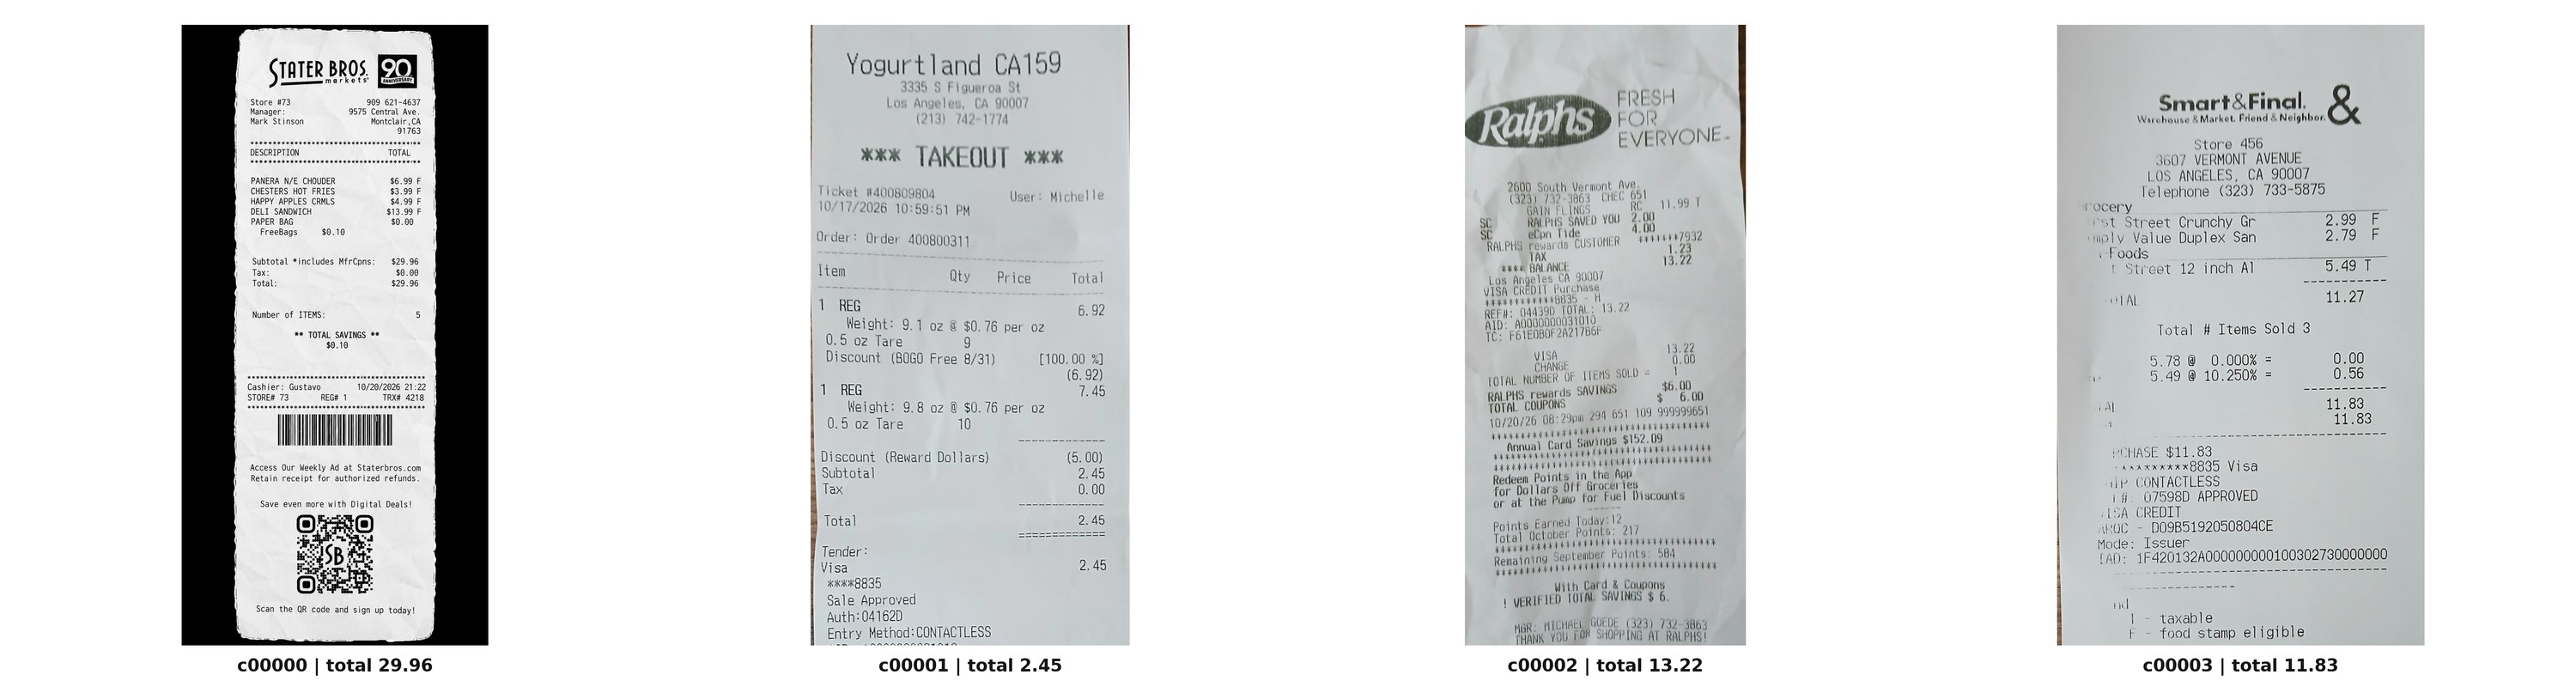
\includegraphics[width=0.5\linewidth]{images/collected_receipts.jpg}\par\raggedright

\end{actcard}
\gap
\begin{card}
\sect{3}{The attack works}
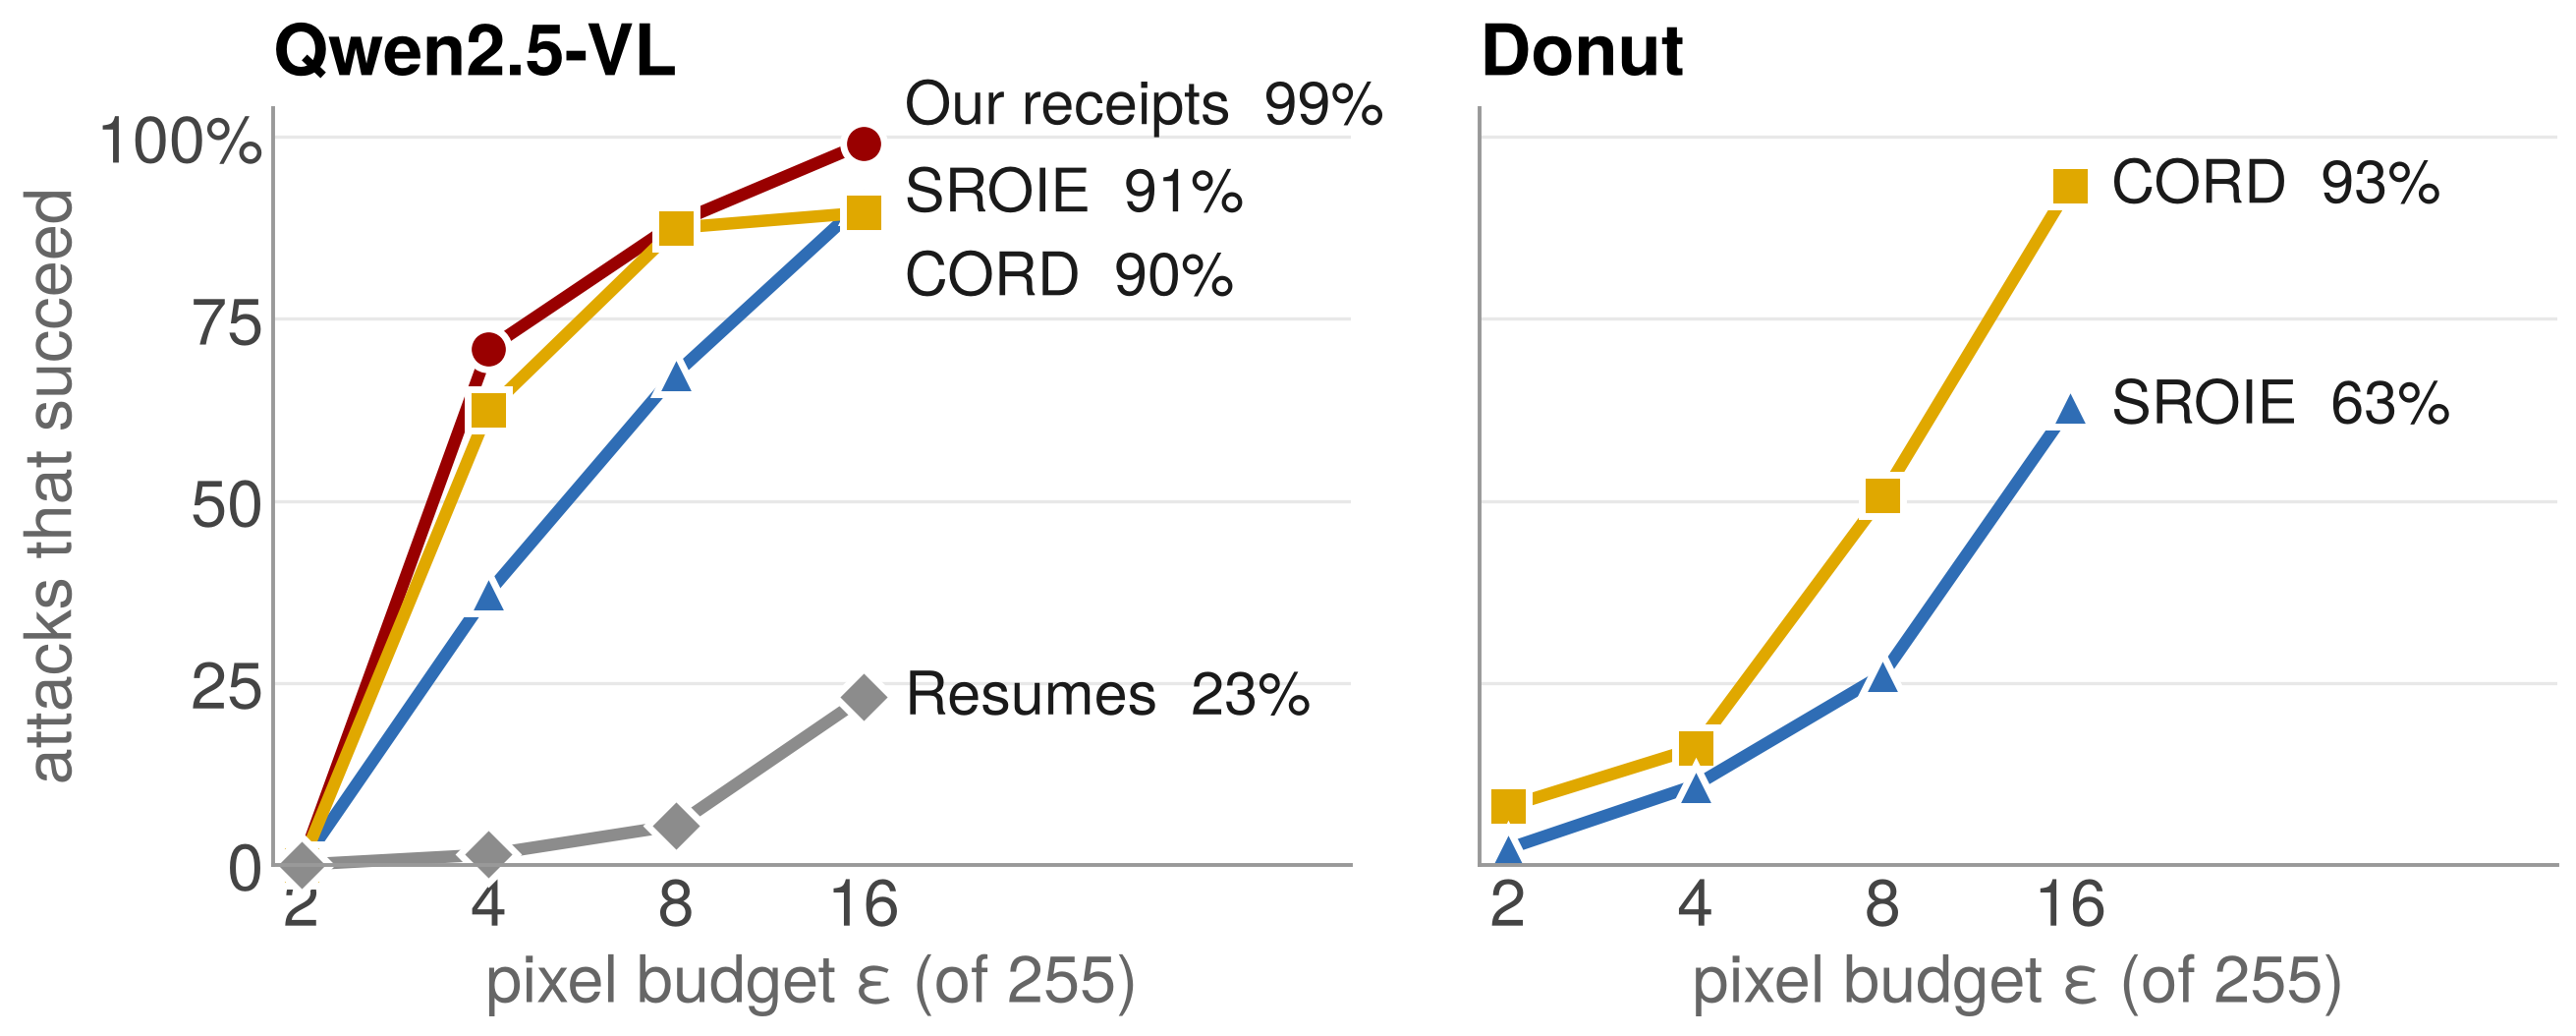
\includegraphics[width=\linewidth]{figures/c_asr.png}
\vspace{3mm}

At the largest budget the attacker's total comes back on \textbf{63--99\% of receipts}. Resumes are harder (23\%): a whole word has to change, not one digit.
\vspace{2mm}

\note{Larger budgets are easier to see: image similarity (SSIM) drops from 0.99 at $\epsilon=2$ to 0.54 at $\epsilon=16$.}
\end{card}
\gap
\begin{card}
\sect{4}{Cleaning the image fails}
JPEG, resizing, voting over several views and re-worded questions blunt a plain attack. An attack that optimizes \emph{through} them (EOT) beats all four at once:
\vspace{4mm}

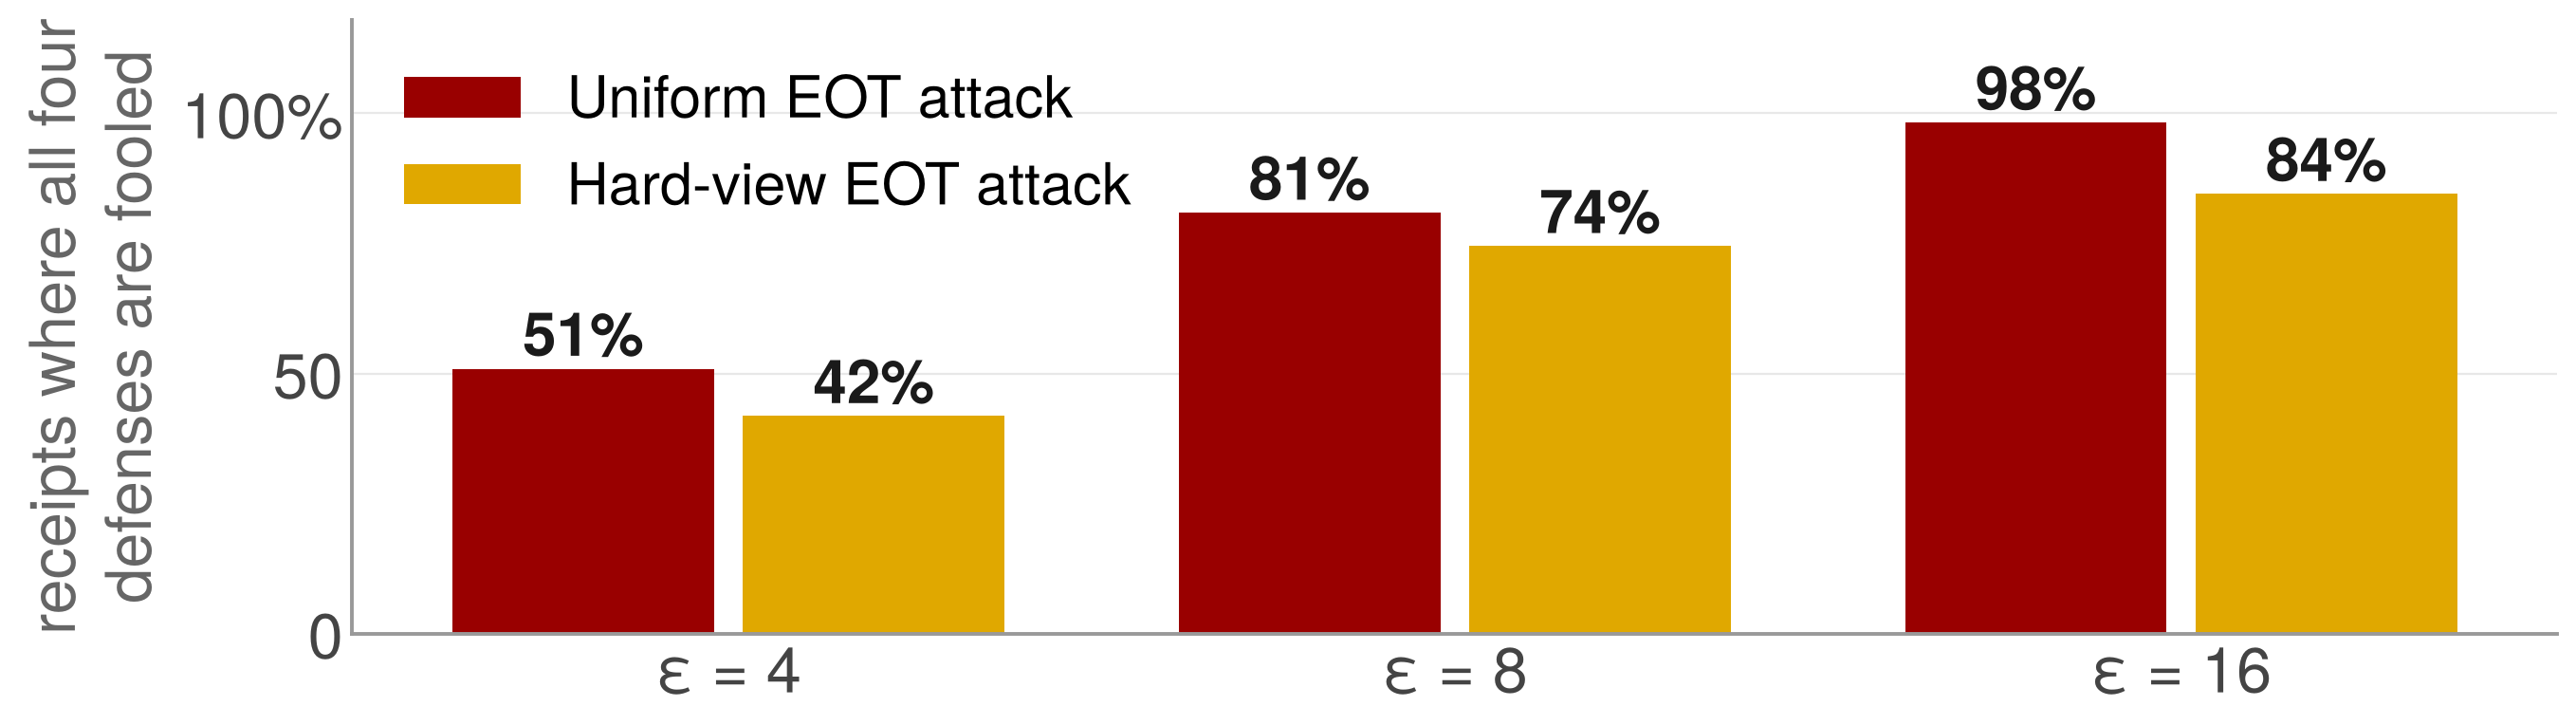
\includegraphics[width=\linewidth]{figures/c_eot.png}
\end{card}
}}

% ---------- column 2: the defense ----------
\posterbox[colback=Page, left=0pt, right=0pt, top=0pt, bottom=0pt, valign=top]{name=col2, column=2, row=11, rowspan=26}{
\vbox to \tcbtextheight{
\begin{actcard}{ACT II}{The defense}
\sect{5}{All 12 defenses, same 396 attacks}
Every method we ran on the held-out receipts, grouped by idea. The right-hand column counts how often the attacker's total got through.
\vspace{4mm}

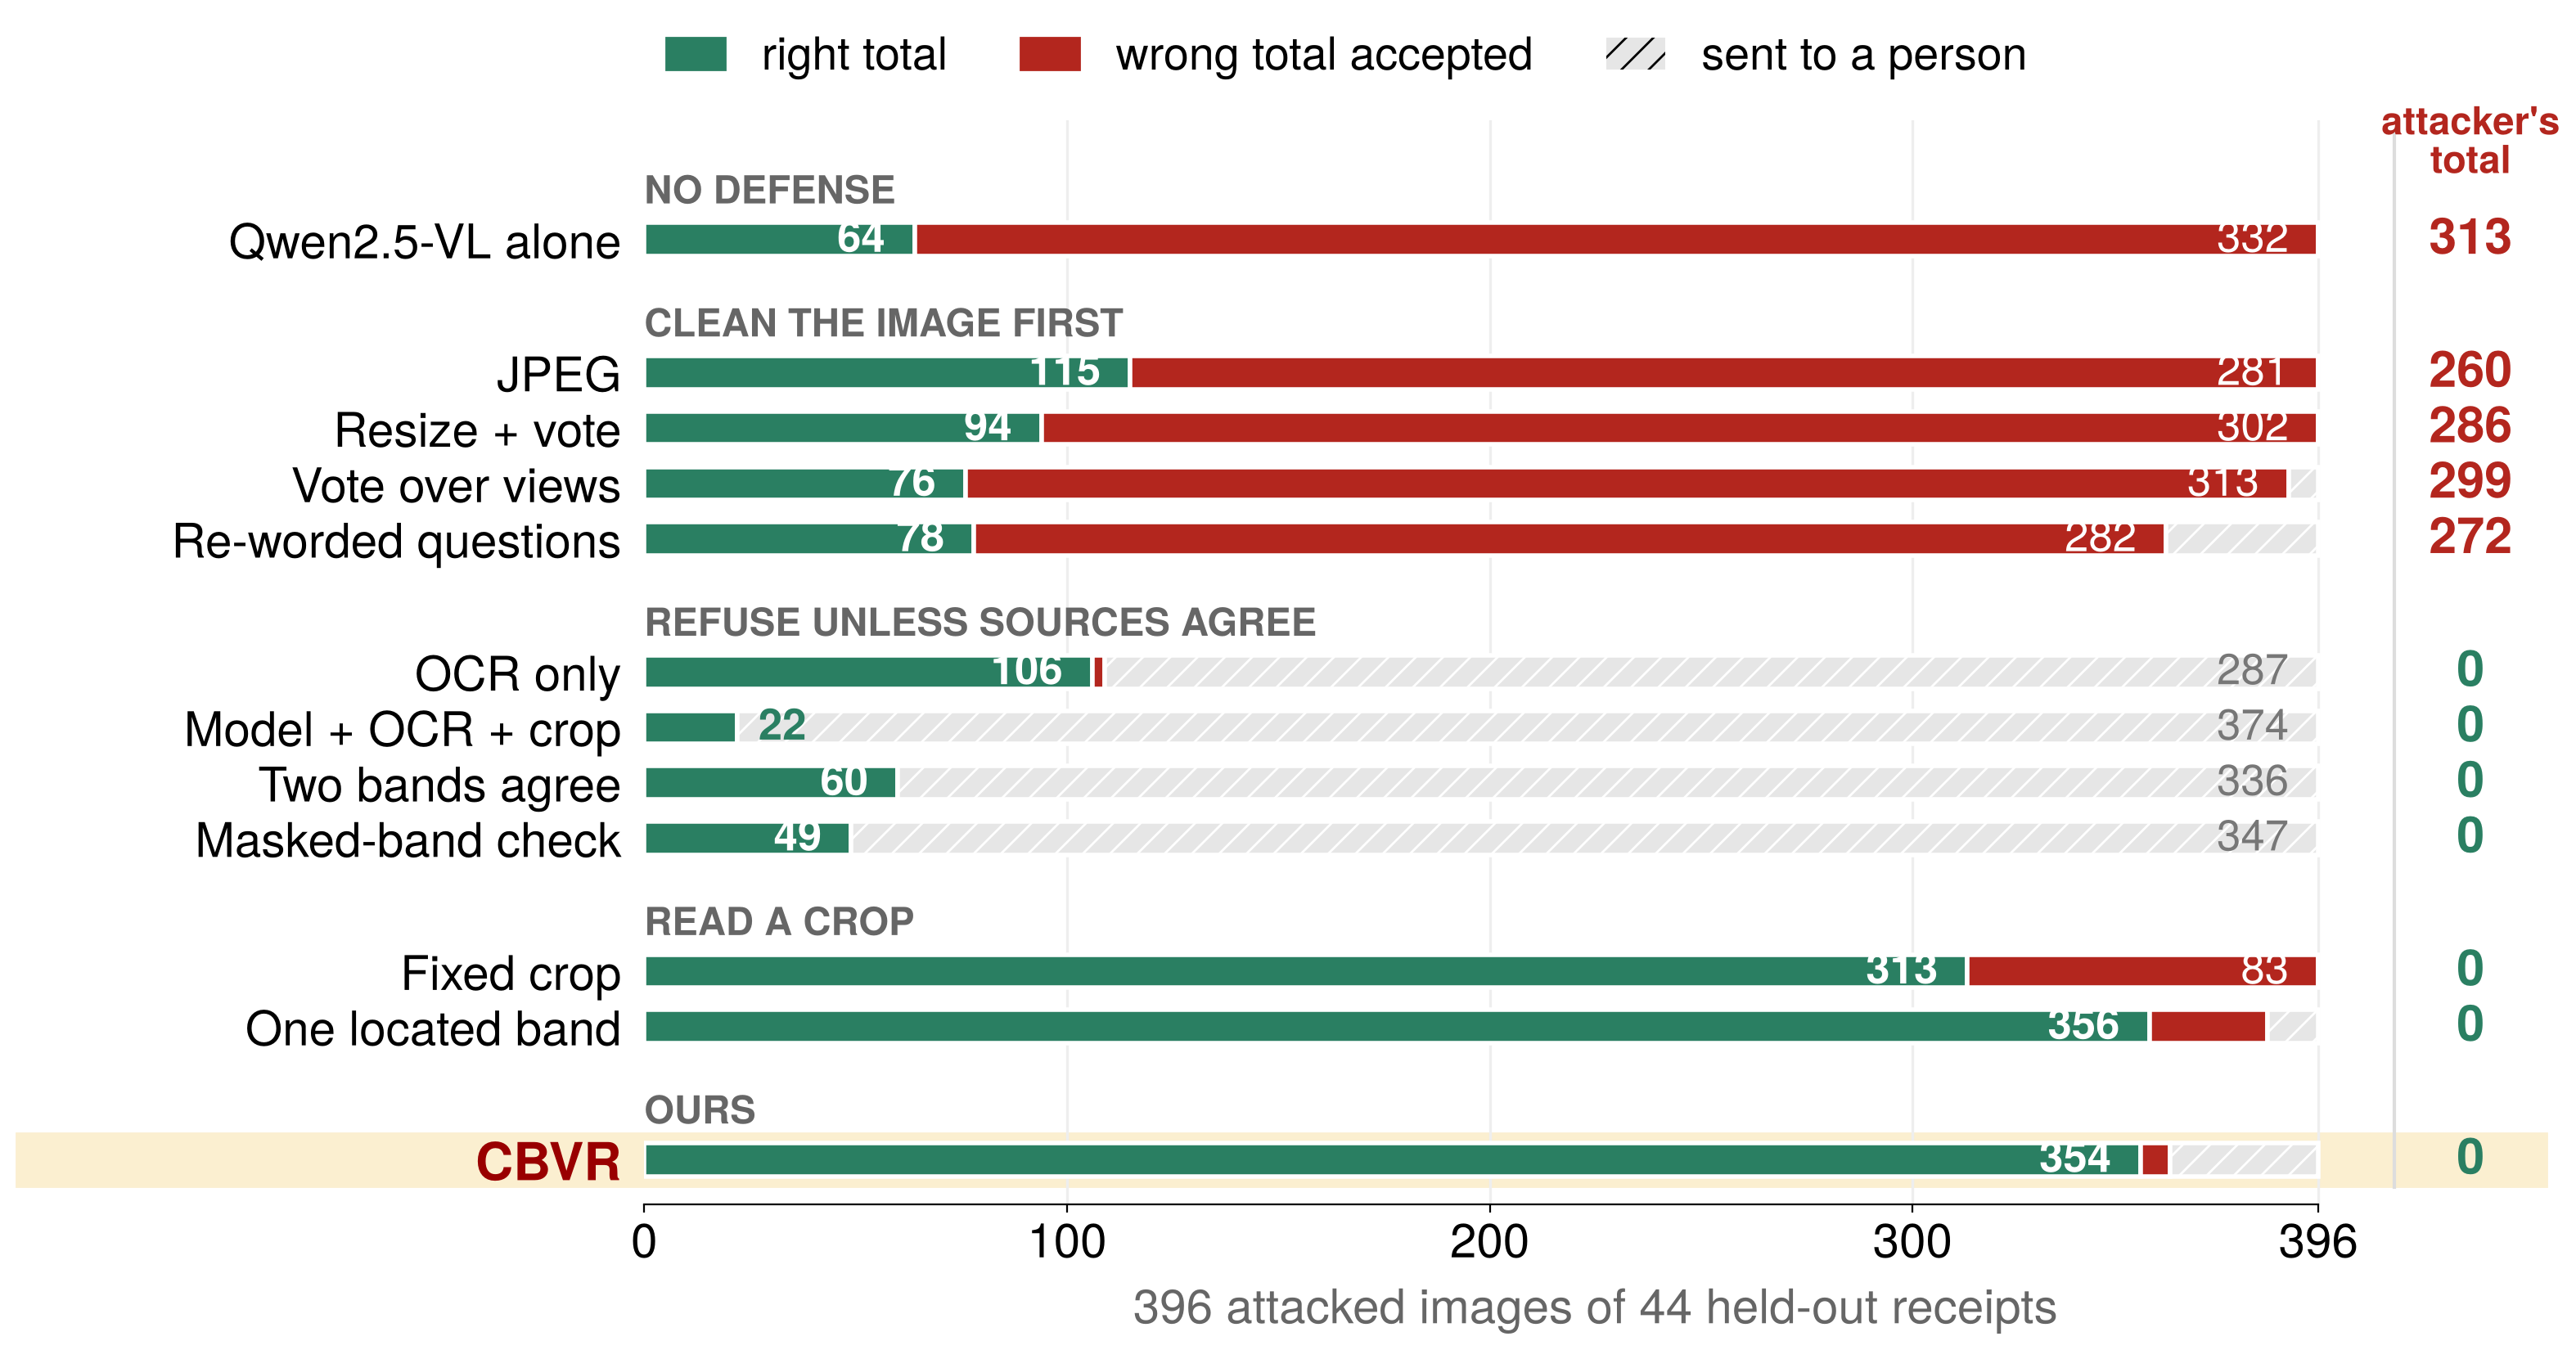
\includegraphics[width=\linewidth]{figures/c_results12.png}
\vspace{4mm}

\begin{itemize}
  \item \textbf{Cleaning} keeps the attacker winning: 260--299 times.
  \item \textbf{Refusing} stops it, but answers only 22--106 times.
  \item \textbf{CBVR} answers right 354 times, and none of its 7 errors is the attacker's total. One band alone accepts 4$\times$ more errors (28).
  \item Cost on 45 clean receipts: 39 right, 1 wrong, 5 refused (no defense: 44, 1, 0).
\end{itemize}
\end{actcard}
\gap
\begin{card}
\sect{6}{It holds for every attack type}
{\fontsize{24}{30}\selectfont
\renewcommand{\arraystretch}{1.3}
\rowcolors{2}{TableAlt}{white}
\begin{tabular}{@{}>{\hspace{2mm}\raggedright\arraybackslash}p{0.36\linewidth}>{\centering\arraybackslash}p{0.28\linewidth}>{\centering\arraybackslash}p{0.28\linewidth}@{}}
\toprule
\rowcolor{TableHead}\textbf{132 images each} & \textbf{No defense right} & \textbf{\textcolor{Cardinal}{CBVR right}} \\
\midrule
Standard attack & \bad{15} & \good{115} \\
Uniform EOT & \bad{19} & \good{121} \\
Hard-view EOT & \bad{30} & \good{118} \\
\bottomrule
\end{tabular}}

\end{card}
\gap
\begin{card}
\sect{7}{Where CBVR still misses}
Of 396 attacks, CBVR missed 42: \textbf{35 sent to a person} (21 with one band right, 12 with no usable band, 2 with both wrong) and \textbf{7 confident errors}.
\vspace{5mm}

\begin{minipage}[t]{0.485\linewidth}
  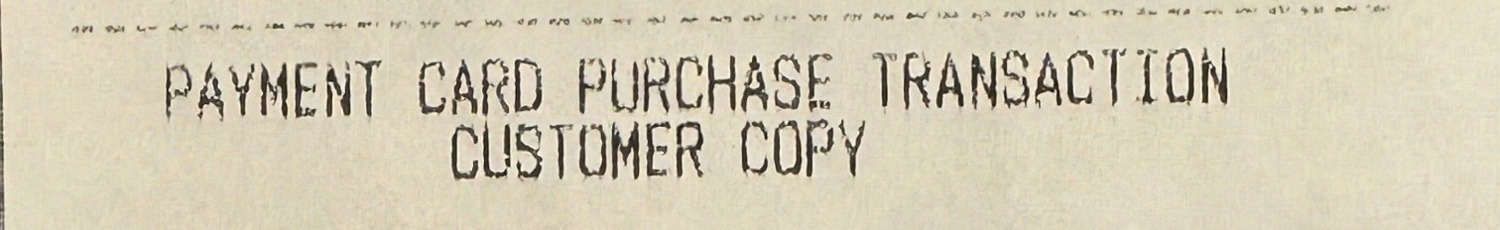
\includegraphics[width=\linewidth,height=30mm,keepaspectratio]{images/b_c00050.jpg}\\[2mm]
  {\fontsize{21}{25}\selectfont\textbf{Refused.} Bands read 12.99 and 4.99, so a person checks.}
\end{minipage}\hfill
\begin{minipage}[t]{0.485\linewidth}
  
\includegraphics[width=\linewidth,height=30mm,keepaspectratio]{images/b_c00071.jpg}\\[2mm]
  {\fontsize{21}{25}\selectfont\textbf{Error.} Both bands read \bad{7133.00} for 71.33.}
\end{minipage}
\vspace{4mm}

\end{card}
}}

% ---------- column 3: stress test ----------
\posterbox[colback=Page, left=0pt, right=0pt, top=0pt, bottom=0pt, valign=top]{name=col3, column=3, row=11, rowspan=26}{
\vbox to \tcbtextheight{
\begin{actcard}{ACT III}{We attack our own defense}
\sect{8}{An attack aimed at CBVR}
A real attacker would know about CBVR. So we optimized against \textbf{both bands at once}: 19 receipts fixed in advance, $\epsilon = 4$ and $8$, two tries each, 100 steps + 100 queries per try.
\vspace{4mm}

{\fontsize{24}{28}\selectfont\bfseries Before}\hfill{\fontsize{24}{28}\selectfont both bands read \good{34.95}}\\[2mm]
\centering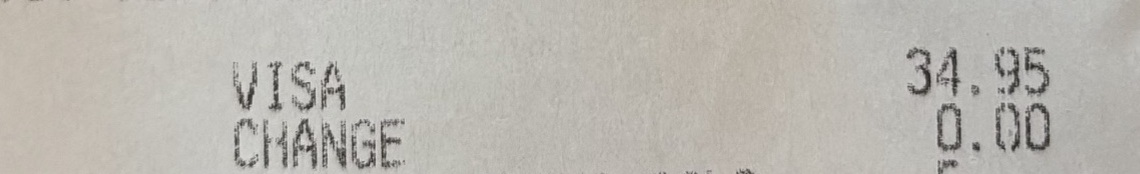
\includegraphics[width=0.6\linewidth]{images/break_clean.jpg}\par\raggedright\vspace{4mm}
{\fontsize{24}{28}\selectfont\bfseries After, $\epsilon = 8$}\hfill{\fontsize{24}{28}\selectfont both bands read \bad{349.50}}\\[2mm]
\centering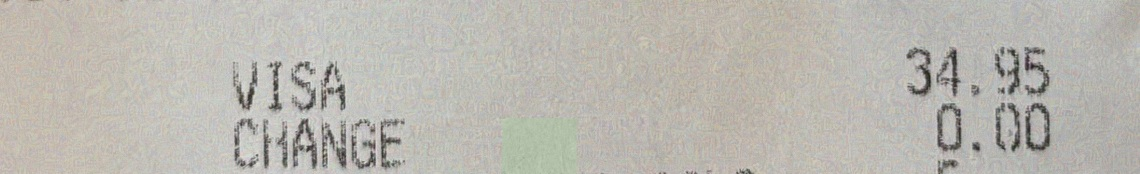
\includegraphics[width=0.6\linewidth]{images/break_attacked.jpg}\par\raggedright
\vspace{6mm}

\centering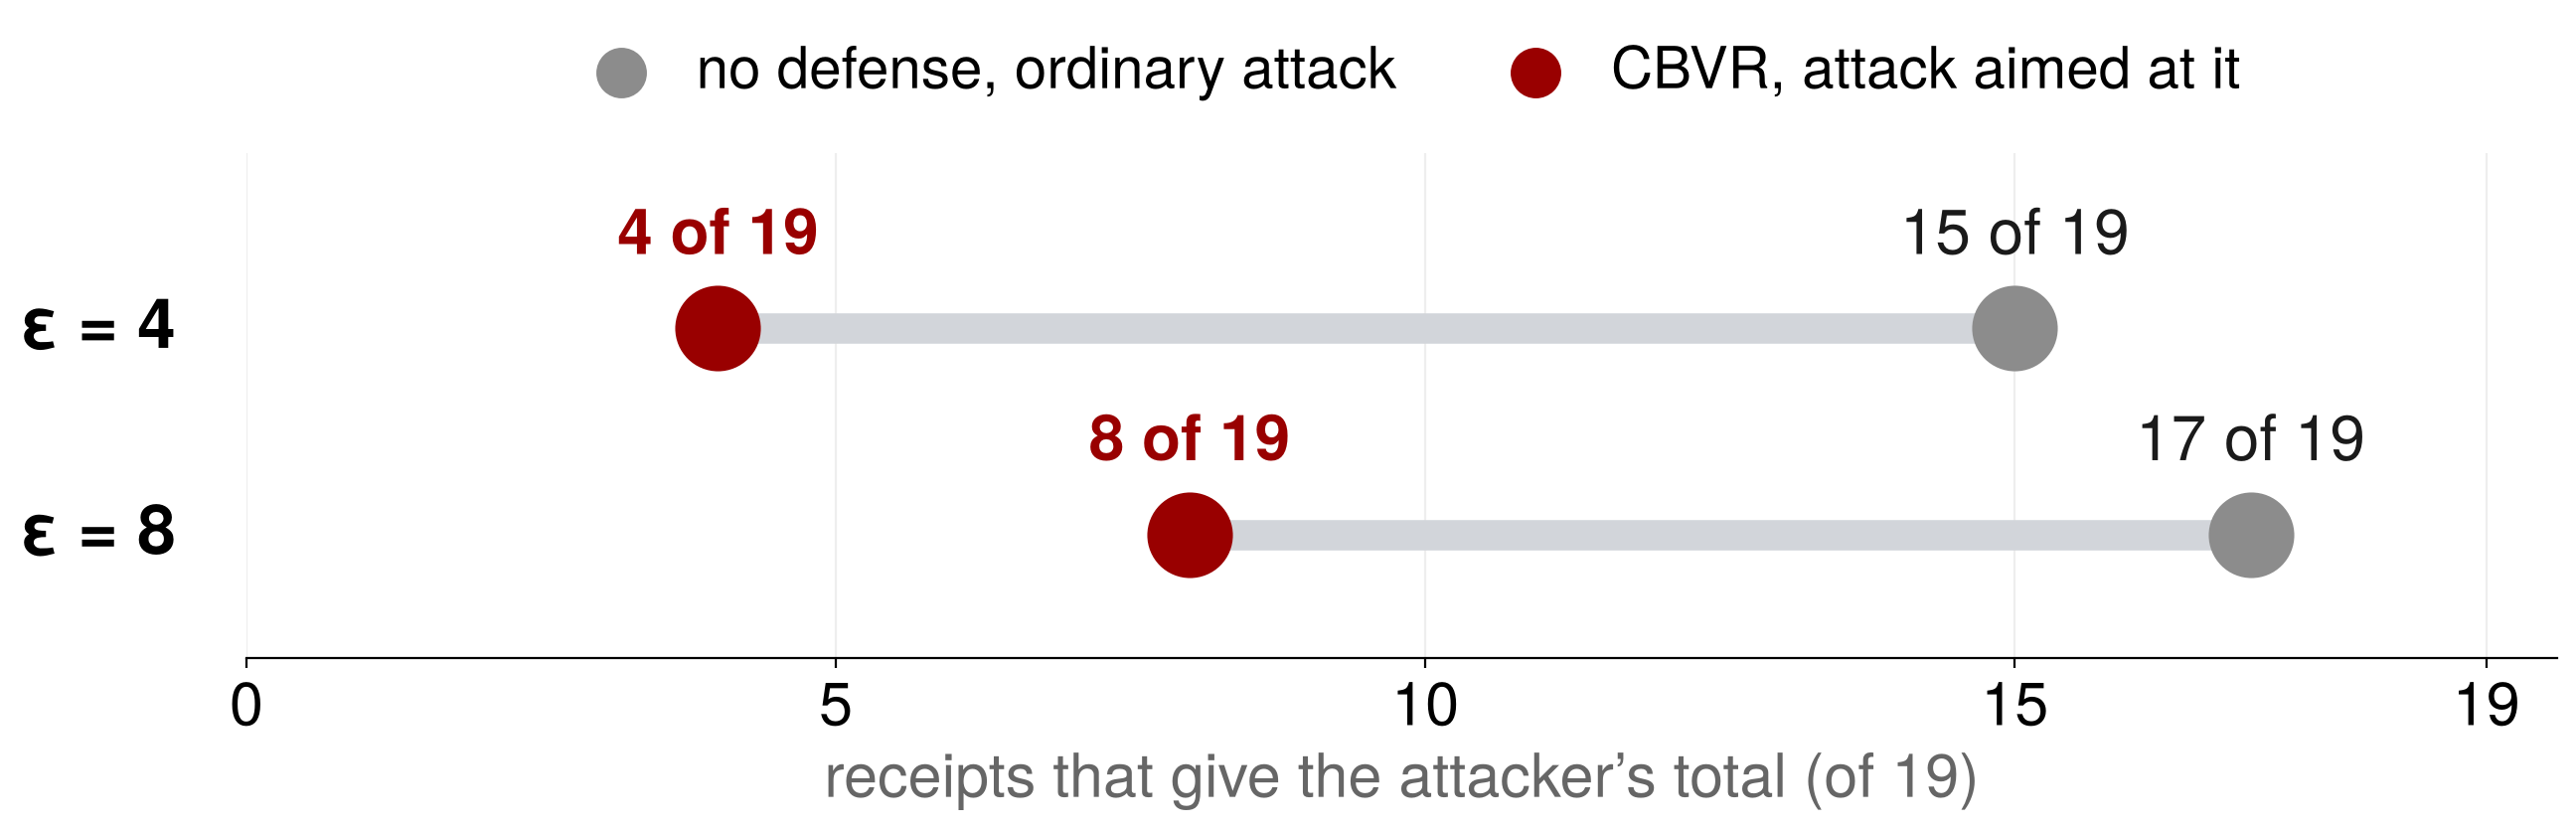
\includegraphics[width=0.8\linewidth]{figures/c_adaptive.png}\par\raggedright
\vspace{3mm}

\textbf{CBVR raises the bar but does not remove it:} 8 of 19 receipts broke at $\epsilon=8$ (95\% CI 23--64\%), against 17 of 19 with no defense. Both bands overlap and share one model, so one pattern can fool both.
\end{actcard}
\gap
\begin{card}
\sect{9}{Every receipt we attacked}
The band CBVR read on each of the 19 receipts (the tight band; for the first, its taller band, because the total sits just above the tight one). Red frame: the attacker's total got through at least once. \textbf{11 never broke}; every other try returned the true total.
\vspace{4mm}

\centering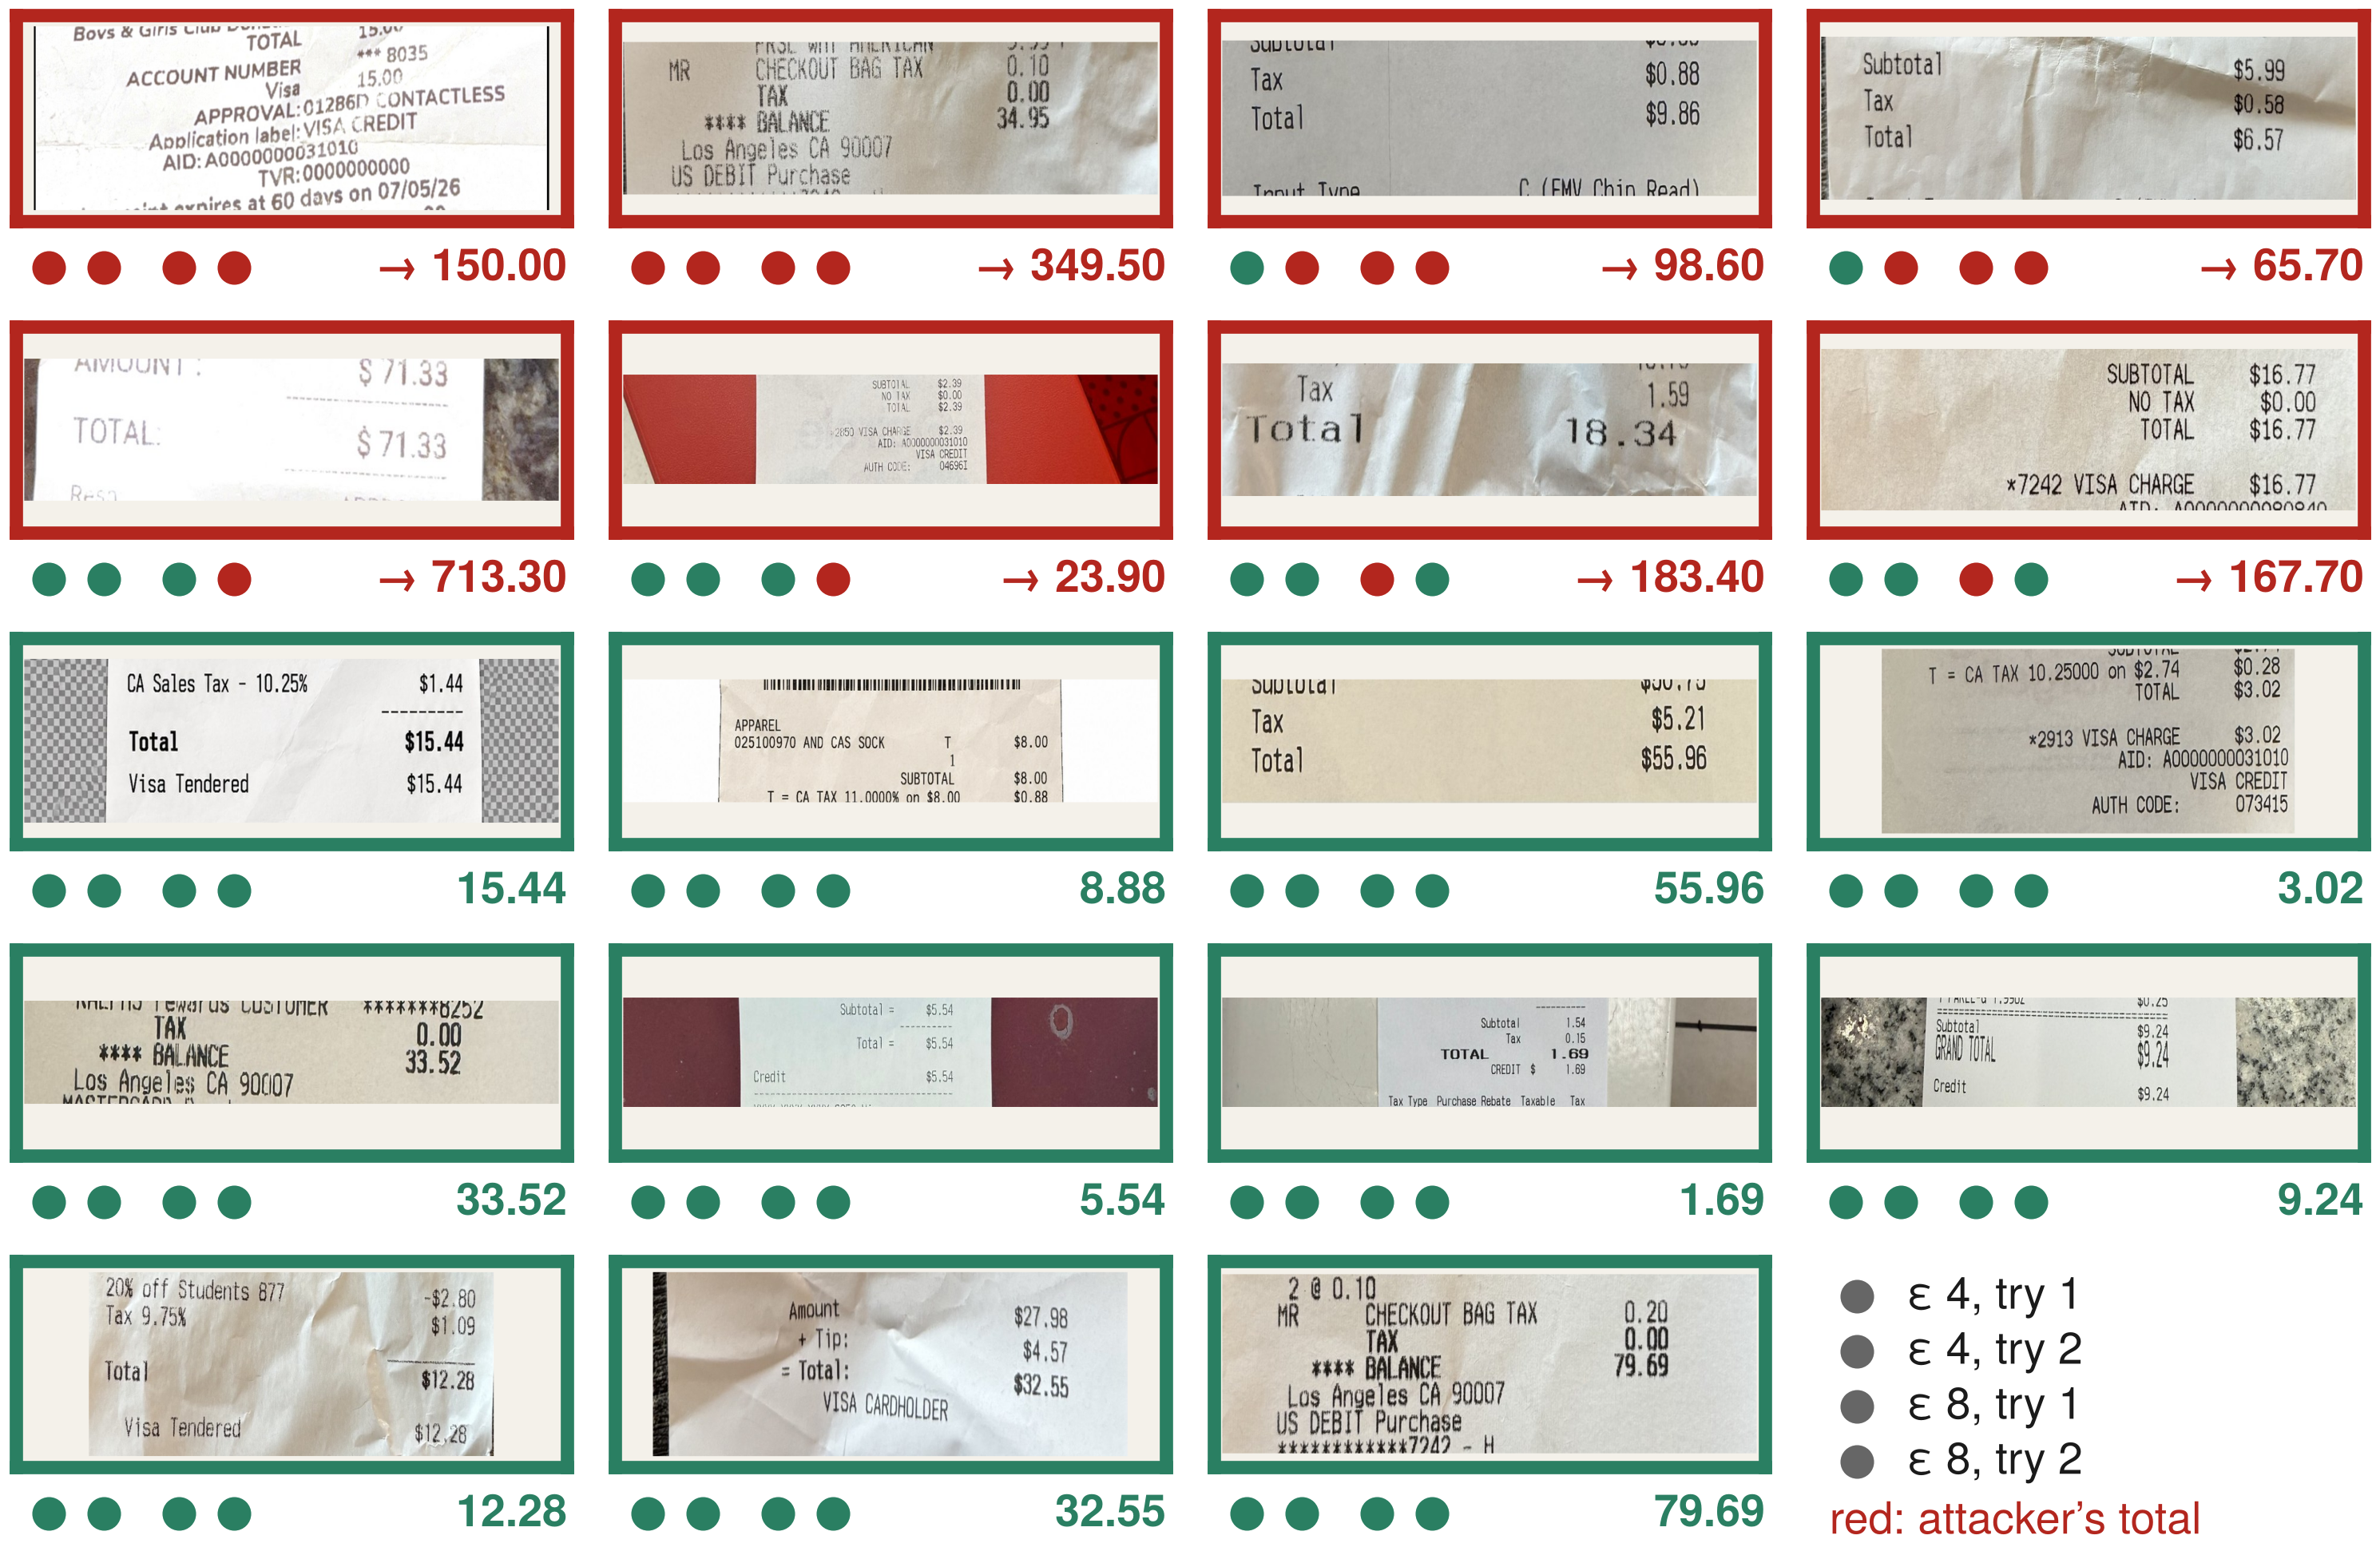
\includegraphics[width=0.9\linewidth]{figures/c_wall19.png}\par
\end{card}
}}

% ---------- column 4: resumes and lessons ----------
\posterbox[colback=Page, left=0pt, right=0pt, top=0pt, bottom=0pt, valign=top]{name=col4, column=4, row=11, rowspan=26}{
\vbox to \tcbtextheight{
\begin{actcard}{ACT IV}{Beyond receipts}
\sect{10}{Resumes held up}
\begin{minipage}[t]{0.48\linewidth}\raggedright
{\fontsize{56}{60}\selectfont\bfseries\color{Bad}22\,\color{Mute}$\rightarrow$\,\color{Good}1}\par\vspace{2mm}
wrong degrees accepted on 236 saved attacks, no defense vs CBVR
\end{minipage}\hfill
\begin{minipage}[t]{0.48\linewidth}\raggedright
{\fontsize{56}{60}\selectfont\bfseries\color{Good}0\,\color{Mute}of\,\color{Ink}40}\par\vspace{2mm}
attacks aimed at CBVR returned the fake degree (10 resumes, $\epsilon$ 8 and 16)
\end{minipage}
\vspace{7mm}

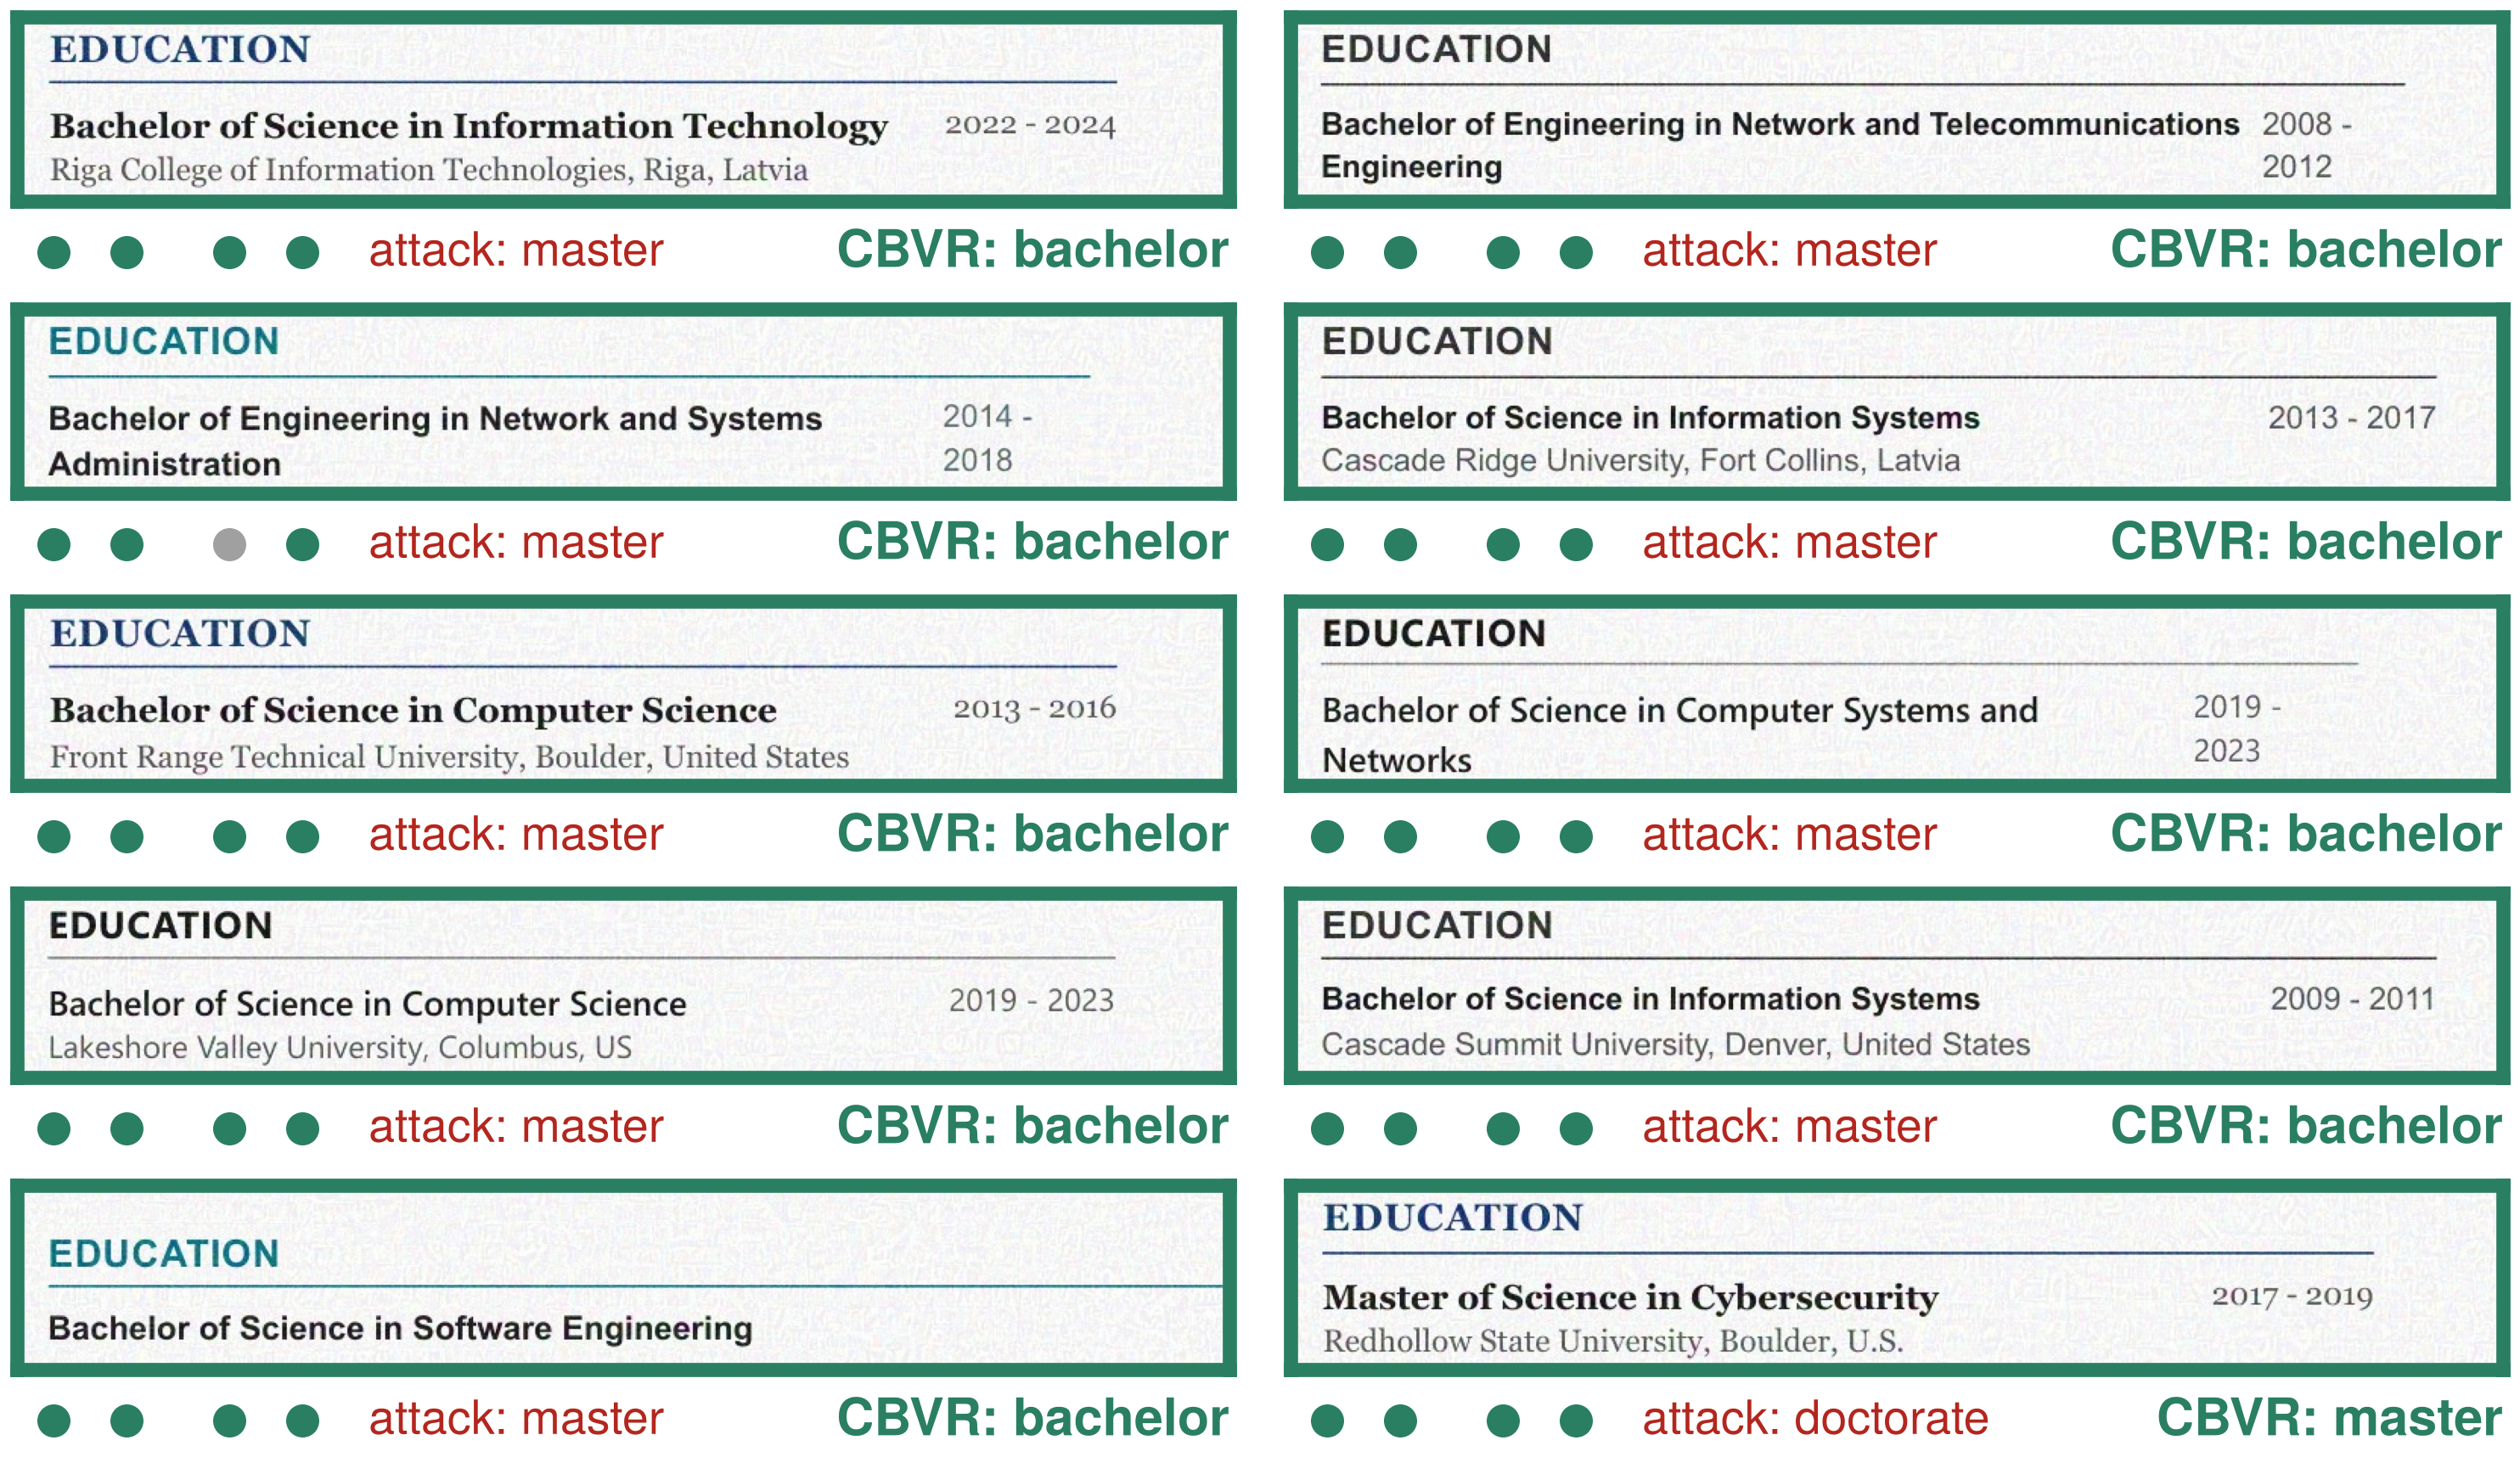
\includegraphics[width=\linewidth]{figures/c_reswall.png}
\vspace{2mm}

\note{Education section of each resume after the strongest attack ($\epsilon=16$). Red: the degree the attack tried to plant. Dots: $\epsilon$ 8 tries 1--2, $\epsilon$ 16 tries 1--2; green: true degree returned, grey: sent to a person.}
\vspace{5mm}

\textbf{Why resumes resist.} The fake answer must replace a whole word (bachelor $\rightarrow$ master), not add one digit; even undefended, ordinary attacks reach only 23\% at $\epsilon=16$; and the education band is large, so the pattern is spread thin.
\end{actcard}
\gap
\begin{card}
\sect{11}{What we learned}
\begin{itemize}
  \item \textbf{Pixel attacks on document AI are practical}, even on fresh phone photos, and far easier on numbers than on words.
  \item \textbf{Re-reading the evidence beats cleaning the image.} CBVR recovers the true total instead of only refusing.
  \item \textbf{Attack your own defense.} Saved attacks never got their total past CBVR; attacks aimed at it broke 8 of 19 receipts.
  \item \textbf{Count three outcomes:} right, wrong, refused. ``No attack succeeded'' can just mean ``everything refused''.
\end{itemize}
\vspace{3mm}

\note{\textbf{Limits.} Attacks were built on one reader (Qwen2.5-VL-3B) and are bounded, not a proof of robustness. With Donut reading, the attacks did not transfer, so CBVR only cost answers (344 $\rightarrow$ 276 right).}
\vspace{4mm}

{\fontsize{20}{25}\selectfont\color{Ink}
\textbf{References.}
Pintore et al., Counterfeit Answers, 2026 \textbullet{}
Madry et al., PGD, ICLR 2018 \textbullet{}
Athalye et al., Synthesizing Robust Adversarial Examples, ICML 2018 \textbullet{}
Athalye et al., Obfuscated Gradients, ICML 2018 \textbullet{}
Tram\`er et al., On Adaptive Attacks, NeurIPS 2020 \textbullet{}
Bai et al., Qwen2.5-VL, 2025 \textbullet{}
Kim et al., Donut, ECCV 2022.\par}
\end{card}
}}

\end{tcbposter}
\end{document}